\documentclass[UTF8]{ctexart}
\usepackage{color}
\usepackage{algorithm}  
\usepackage{algpseudocode}  
\usepackage{amsmath}  
\renewcommand{\algorithmicrequire}{\textbf{Input:}}
\renewcommand{\algorithmicensure}{\textbf{Output:}}

\usepackage{tikz}
\usepackage{verbatim}
\usetikzlibrary{trees}

\title{字符串匹配算法及其衍生ACM问题的探究}
\author{余畅, 2019091621002}
\begin{document}
\maketitle

\section{摘要}
\textbf{关键词:字符串匹配, Brute-Force, Knuth-Morris-Pratt, Tire, Aho-Corasick automaton, Suffix Tree/Automaton} \par
\textbf{字符串匹配}的各种形式(如单模式串单目标串、多模式串单目标串、目标串子区间模式匹配)及其衍生的DP、区间求值问题,因其思维要求有较强的层次性,一直是ACM竞赛中的常驻考点和热点。不同的字符串匹配算法和数据结构,也在不同层次的ACM题目中发挥着不同的作用。\par
本论文旨在探究几种ACM中字符串匹配的常用的算法和数据结构:\textbf{Brute-Force算法}、\textbf{Knuth-Morris-Pratt算法}、\textbf{Tire树算法}、\textbf{Aho-Corasick Automaton算法}、\textbf{Suffix Tree算法}和\textbf{Suffix Automaton算法},分析其算法过程,时空复杂度和适用范围,并对论文中提出的几道字符串例题予以解决。

\section{问题背景}

\textbf{模式串匹配}(String Pattern Matching)是数据结构中字符串的一种基本运算,给定一个子串,要求在某个字符串中找出与该子串相同的所有子串。然而问题的基本性和问题的复杂度并不成比例。对于最朴素的算法,其复杂度在给定的问题规模下往往无法接受:ACM中所遇到的有关字符串匹配的问题,其目标串规模往往在$10^5$乃至$10^6$的级别,模式串给出的形式更是五花八门,串长或者串的数量单个指标都能达到$10^5$的级别,而且往往要求强制在线,即只能对主串进行预处理。一些在单纯匹配问题上优越的算法,遇到了结合DP,区间求值等符合问题时,又往往有其局限性,即无法按照题目要求划分问题,并在合理的时空复杂度中进行数据保存和状态转移。 \par
本论文旨在同时探究,并试图解决这两个问题:\textbf{更优越的时空复杂度和更广泛的适用范围}。

\section{算法探究}

\subsection {Brute-Force算法}

\subsubsection {算法描述}

BF算法,即暴力算法,是最普通和朴素的模式匹配算法。其主要思想就是将目标串$S$的第一个字符与模式串$T$的第一个字符进行匹配,若相等,则继续比较$S$的第二个字符和$T$的第二个字符;若不相等,则比较$S$的第二个字符和$T$的第一个字符,依次比较下去,直到得出最后的匹配结果。具体的伪代码可见\textbf{算法1}。

\begin{algorithm}
\caption{Brute-Force}  
\label{alg:Brute-Force}  
\begin{algorithmic} [1]
    \Require  
      Target String, $S$;
	  Pattern String, $T$
    \Ensure  
      First matched position: $Pos$;  
    \Function {Brute-Force}{$S$, $T$}
		\State $N \gets \Call{length}{S}$
		\State $M \gets \Call{length}{T}$  
		
		\For{$i = 0 \to N - M$}
			\State Boolean $Flag \gets True$
			\For{$j = 0 \to M - 1$}
				\If{$S[i+j] \ne T[j]$}
					\State $Flag \gets False$
					\State \textbf{break}
				\EndIf
			\EndFor
			\If{$Flag = True$}
				\State \Return $i$ where Match first successful
			\EndIf
		\EndFor
	\State \Return $-1$ where Match failed
	\EndFunction  
\end{algorithmic}
\end{algorithm}

\subsubsection {算法分析}

对算法稍加改动,即可让算法匹配目标串中所有的模式串。但从两重循环分析可知,Brute-Force算法无论是单次匹配还是多次匹配,其复杂度最坏情况下都是$\mathcal{O}(N \cdot M)$,这决定了其作为暴力算法注定无法用在高难度题目的正确解法上。但是对于不以字符串匹配为主要考点而是将其作为程序某部分预处理的工具,Brute-Force算法因其简单的写法还是有其用武之地。 \par
值得注意的是,当模式串长度$M$远小于$N$或者极其接近$N$时,哪怕是最坏复杂度也会退化为$\mathcal{O}(N)$;此外,当出题人偷懒而没有精妙地构造$S$和$T$时(即用随机数生成字符串),由于随机串的性质,每一轮的匹配往往经过极其有限次比较就失配,使得复杂度退化为$\mathcal{O}(N+M)$,因此作为暴力骗分算法也未尝不可。

\subsection {Knuth-Morris-Pratt 算法}

\subsubsection {算法描述}

Brute-Force算法最大的问题就是:当前的匹配一旦\textbf{失配}以后,主串的指针会重新回溯到开头重新进行下一轮的比较。但实际上,当前轮和上一轮的比较往往有许多重复,基于上一轮已经匹配所得到的信息,我们希望能够节省新一轮所匹配的次数,这时需要引入的就是KMP算法。 \par
KMP 算法是 D.E.Knuth、J,H,Morris 和 V.R.Pratt 三位前辈共同提出的,称之为 Knuth-Morria-Pratt 算法,简称 KMP 算法。该算法相对于 Brute-Force算法的改进之处,就是利用\textbf{已知信息}消除了主串指针的回溯,从而使算法效率提升到了新的境界。现在引入的第一个需要解决的问题是,这个\textbf{已知信息}究竟是指什么,让我们先来观察一个匹配过程:\par
\begin{itemize}
  \item [1)] 
  主串"\textcolor[rgb]{1,0,0}{B}BC ABCDAB ABCDABCDABDE"的第一个字符与模式串"\textcolor[rgb]{1,0,0}{A}BCDABD"的第一个字符,进行比较。因为B与A不匹配,所以模式串后移一位。
  \item [2)]
  "B\textcolor[rgb]{1,0,0}{B}CABCDABABCDABD", "\textcolor[rgb]{1,0,0}{A}BCDABD" 因为B与A不匹配,模式串再往后移一位。
  \item [3)]
  "BBC\textcolor[rgb]{1,0,0}{A}BCDABABCDABD", "\textcolor[rgb]{1,0,0}{A}BCDABD" 进行上述操作,直到主串有一个字符,与模式串的第一个字符相同。
  \item [4)]
  "BBC\textcolor[rgb]{1,0,0}{AB}CDABABCDABD", "\textcolor[rgb]{1,0,0}{AB}CDABD" 继续比较主串和模式串的下一个字符,还是相同。
  \item [5)]
  "BBC\textcolor[rgb]{1,0,0}{ABCDAB}\textcolor[rgb]{0,0,1}{A}BCDABD", "\textcolor[rgb]{1,0,0}{ABCDAB}\textcolor[rgb]{0,0,1}{D}" 进行上述操作,直到主串有一个字符,与模式串对应的字符不相同。
  \item [6)]
  "BBCA\textcolor[rgb]{1,0,0}{B}CDABABCDABD", "\textcolor[rgb]{1,0,0}{A}BCDABD" 这时,如果按照BF算法的思路,将模式串整个后移一位,再从头逐个比较。这样做虽然可行,但是效率很差,因为你要把"搜索位置"移到已经比较过的位置,重比一遍。
  \item [7)]
  "BBC\textcolor[rgb]{1,0,0}{ABCDAB}\textcolor[rgb]{0,0,1}{A}BCDABD", "\textcolor[rgb]{1,0,0}{ABCDAB}\textcolor[rgb]{0,0,1}{D}" 一个基本事实是,当A与D不匹配时,你其实知道前面六个字符是"ABCDAB"。KMP算法的想法是,设法利用这个已知信息,不要把"搜索位置"移回已经比较过的位置,继续把它向后移,这样就提高了效率。
\end{itemize}


\begin{algorithm}
\caption{Get-Next-Array}  
\label{alg:KMP get Next-Array}  
\begin{algorithmic} [1]
    \Require  
	  Pattern String: $T$
    \Ensure  
      Next-Array: $next$;  
    \Function {Get-Next-Array}{$next[]$, $T$}
		\State $j \gets 0$
		\State $k \gets -1$
		\State $next[0] \gets -1$
		\While{$j < \Call{length}{T} - 1$}
			\If{$k = -1$ \textbf{or} $t[j] = t[k]$}
				\State $j++$
				\State $k++$
				\State $next[j]=k$
			\Else 
				\State $k=next[k]$
			\EndIf
		 \EndWhile
	\EndFunction  
\end{algorithmic}
\end{algorithm}

这时,用到的\textbf{已知信息}即是:对于每模式串 $t$ 的每个元素 $t_j$,都存在一个实数 $k$ ,使得模式串 $t$ 开头的 $k$ 个字符($t_0$ $t_1$…$t_{k-1}$)依次与 $t_j$ 前面的 $k$($t_{j-k}$ $t_{j-k+1}$…$t_{j-1}$,这里第一个字符 $t_j-k$ 最多从 $t_1$ 开始,所以 $(k < j)$个字符相同。如果这样的 $k$ 有多个,则取最大的一个。模式串 $t$ 中每个位置 $j$ 的字符都有这种信息,采用 $next$ 数组表示,即 $next[j]=MAX\{ k \}$


总结来说,\textbf{已知信息},也即\textbf{部分匹配值},就是模式串某一前缀自身(包括这个字符串本身)的前缀和自身后缀的最长的共有元素的长度。 \par 

例"ABCDABD",就可以由"A","AB","ABC","ABCD","\textcolor[rgb]{1,0,0}{A}BCD\textcolor[rgb]{1,0,0}{A}","\textcolor[rgb]{1,0,0}{AB}CD\textcolor[rgb]{1,0,0}{AB}","ABCDABD" 等前缀得到其$next=\{0, 0, 0, 0, 1, 2, 0\}$

如果只通过上述朴素的思想来求$next$数组的话,时间复杂度会达到$\mathcal{O}(M^2)$,然而我们可以通过以上的\textbf{算法2},使得复杂度降为$\mathcal{O}(M)$。

此处分析\textbf{算法2}的求解过程:\par
\begin{itemize}
  \item [1)] 特殊情况 \par 
	当 $j$ 的值为 $0$ 或 $1$ 的时候,它们的 $k$ 值都为 $0$,即 $next[0] = 0$,$next[1] =0$。但是为了后面 $k$ 值计算的方便,我们将 $next[0]$ 的值设成 $-1$。
 \item [2)] $t[j]=t[k]$ \par
	假设字符串"\textcolor[rgb]{1,0,0}{AB}C\textcolor[rgb]{0,0,1}{AB}CD", $k=2$, $j=5$(下标从 $0$ 开始)。 
	\par 观察可知,当 $t[j] = t[k]$ 时,必然有$"t[0] \to t[k-1]" = " t[j-k] \to t[j-1]"$,此时的 $k$ 即是相同子串的长度。因为有$"t[0] \to t[k-1]" = " t[j-k] \to t[j-1]"$,且 $t[j] = t[k]$,则有$"t[0] \to t[k]" = " t[j-k] \to t[j]"$,也就得出了$next[j+1]=k+1$。
 \item [3)] $t[j] \ne t[k]$ \par
	假设字符串"\textcolor[rgb]{1,0,0}{ABA}CDA\textcolor[rgb]{0,0,1}{BAB}C", $k=3$, $j=8$(下标从 $0$ 开始)。
	\par 观察可知,当 $t[j] = t[k]$ 时,$t[j+1]$ 的最大子串的长度为 $k$,即 $next[j+1] = k+1$。但是此时$t[j] \ne t[k]$ 了,所以就有 $next[j+1] < k$,那么求 $next[j+1]$ 就等同于求 $t[j]$ 往前小于 $k$ 个的字符(包括$t[j]$)与 $t[k]$ 前面的字符的最长重合串,即 $t[j-k+1] \to t[j]$ 与 $t[0] \to t[k-1]$ 的最长重合串,那么就相当于求 $next[k]$(只不过 $t[k]$ 变成了 $t[j]$,但是 $next[k]$ 的值与 $t[k]$ 无关)。所以有 $k = next[k]$,如果新的一轮循环(这时 $k = next[k]$ ,$j$ 不变)中 $t[j]$ 依然不等于 $t[k]$ ,则说明倒数第二大 $t[0 \to next[k]-1]$ 也不行,那么 $k$ 会继续被 $next[k]$ 赋值,直到找到符合重合的子串或者 $k = -1$。
\end{itemize}
至此,得到 $next$ 数组之后,已经可以给出KMP的全部实现,伪代码可见下文的\textbf{算法3}:

\begin{algorithm}
\caption{KMP}  
\label{alg:KMP}  
\begin{algorithmic} [1]
    \Require  
      Target String, $S$;
	  Pattern String, $T$
    \Ensure  
      First matched position: $Pos$;  
    \Function {KMP}{$S$, $T$}
		\State $i \gets 0$
		\State $j \gets 0$  
		\State \Call{Get-Next-Array}{next, T}
		\While{$i < \Call{length}{S}$ \textbf{and} $j < \Call{length}{T}$}
			\If{$j = -1$ \textbf{or} $s[i] = t[j]$}
				\State $i++$
				\State $j++$
			\Else 
				\State $j=next[j]$
			\EndIf
		 \EndWhile
	\If{$j >= \Call{length}{T}$}
				\State \Return $i-length(T)$ where Match successful
			\Else 
				\State \Return $-1$ where Match failed
			\EndIf
	\EndFunction  
\end{algorithmic}
\end{algorithm}

\subsubsection {算法分析}
KMP算法分成两部分,第一部分通过模式串 $T$ 求出提供信息的 $next$ 数组,时间复杂度为 $\mathcal{O}(M)$,第二部分为利用 $next$ 数组优化BF算法框架下的匹配过程,使得匹配阶段的时间复杂度降为 $\mathcal{O}(N)$,所以总时间复杂度为$\mathcal{O}(N+M)$,空间复杂度为$\mathcal{O}(M)$。至此,单模式串单目标串的匹配问题已经完美解决。 \par
此外,由于在解决问题的过程中得到了储存匹配信息的 $next$ 数组,而这个数组本身具有很好的性质可以解决一些问题。例如\textbf{HDU3336},题目大意是给定一个字符串$s$,求$s$的每个前缀在此字符串中出现的次数之和。如果只是朴素地枚举前缀,求出每个前缀出现的次数,效率必然无法在规定时间内解决问题,但是利用kmp算法的 $next$ 数组可以很好的解决这个问题。由 $3.2.1节$ 的算法描述可知,$next$ 数组存放的是字符串的前缀和后缀能匹配的字符个数的最大值。对于 $i$:
\begin{itemize}
  \item [1)] $next[i]  = 0$,则由 $s$ 的前 $i$ 个字符组成的字符串的所有后缀肯定和其前缀不匹配。
  \item [2)] $next[i]  \ne 0$,则由 $s$ 的前 $i$ 个字符组成的字符串存在某个前缀和后缀匹配的情况,也就是该前缀的出现的次数应该加上 $1$。
\end{itemize}
从而,我们就可以通过递推的思想解决问题。定义$f_i$为由 $s$ 的前 $i$ 个字符组成的字符串中,所有前缀出现的次数之和。

\begin{equation} 
f_i = f_{i-1} + 1 + (next[i] \ne 0)
\end{equation}

然而,KMP算法也有其局限性,其进行处理的部分是模式串 $T$ 而不是目标串 $S$,而对于每一个模式串 $T$ 的匹配过程,都需要重新对其进行预处理,然后对整个目标串 $S$ 进行遍历。这就意味着进行多模式串匹配的时候,算法的效率就会大大降低;KMP算法对主串的性质也一无所知,如果涉及到主串区间,主串前后缀等需要剖析主串性质的问题时,KMP算法亦无法很好的胜任。KMP算法在ACM竞赛中最重要的思想和价值,在于对其 $next$ 数组进行深刻的理解,然后利用 $next$ 数组的特殊计数性质解决一些KMP相关的字符串问题,而不仅仅是背一个KMP的板子,虽然其代码确实简短容易记忆,但直接考察字符串匹配的裸题,可能性甚微。

\subsection {Trie 树}

在这一章中,让我们暂时抽离模式串匹配这个问题本身,来了解一种新的数据结构,Trie 树(字典树),以便更好地理解后续的一些算法。

\subsubsection {算法描述}

Trie 树(字典树)本质上是一棵$k-$叉树,其中$k$是字典集的大小。不同于二叉树中每个节点存放的是左右孩子的指针,Trie 树中每个节点存放的是一个大小为$k$的数组或者散列表。将一个字符串插入到Trie 树中的方法是从根节点(根节点为字符串的空集)开始,依次通过当前字符找到下一个儿子节点,继续递归访问插入,并在每个访问到的结点上给计数加一,如伪代码\textbf{算法4}所示:

\begin{algorithm}
\caption{Trie-Tree-Insert}  
\label{alg:Trie Tree Insert Algorithm} 
\begin{algorithmic} [1] 
	\Require $T$: Trie-Tree Node; $S$: String; $k$: Current String Index
    \Function {Trie-Tree-Insert}{$T$, $S$, $k$}
	\State $T.count += 1$
		\If{$k = \Call{length}{S} - 1$}
				\State \Return
		\EndIf
		\State $c \gets T.children(S[k])$
		\If{$c = \phi $}
				\State $c \gets $ \Call{New-Node}{c}
		\EndIf
		\State \Call{Trie-Tree-Insert}{c, S, k + 1}
	\EndFunction  
\end{algorithmic}
\end{algorithm}

查找某一前缀出现的次数也同理可得,伪代码\textbf{算法5}所示:

\begin{algorithm}
\caption{Trie-Tree-Search}  
\label{alg:Trie Tree Search Algorithm} 
\begin{algorithmic} [1] 
	\Require $T$: Trie-Tree Node; $S$: String; $k$: Current String Index
    \Function {Trie-Tree-Search}{$T$, $S$, $k$}
		\If{$k = \Call{length}{S} - 1$}
				\State \Return $T.count$
		\EndIf
		\State $c \gets T.children(S[k])$
		\If{$c = \phi $}
				\State \Return $0$
		\EndIf
		\State \Call{Trie-Tree-Search}{c, S, k + 1}
	\EndFunction  
\end{algorithmic}
\end{algorithm}

\subsubsection {算法分析}

Trie 树的时间复杂度是线性的,即$\mathcal{O}(N^*)$,其中 $N^*$ 为插入和查找的字符串的总长度。但是其空间复杂度有一定的局限性:Trie 树仅能在相同前缀的部分共用储存空间,但是如果所插入的字符串前缀差异较大,即树在较前面的地方就产生过多的分支,那么就可能要对所有字符串中的每一个字符都新建一个结点。Trie 树的每个结点又需要保存其$k$个儿子的指针,所以最坏情况下的空间复杂度是$\mathcal{O}(k \cdot N^*)$。

Trie 树有许多很好的性质,因为其相当于合并了所以主串公共前缀的部分,所以只需要一次查找就可以找到某前缀出现的所有次数,而任意两个串所对应的结点的LCA(最近公共祖先)就是其字符串的最长公共前缀。将字符串整理成树的形式,也很容易通过树的遍历,树形DP和树链剖分来解决一些特定的问题。例如\textbf{HDU4825},题目大意是给出 $n$ 个数和 $m$ 次询问,每次询问给出一个数 $x$ ,问在 $n$ 个数中哪个数与 $x$ 异或值最大。

我们可以先将每个数先转化成二进制,也就是 $01$ 字符串,然后补上前导 $0$ 保存在2-Trie 树中。考虑按位异或的形式,如果想让异或的最终结果尽可能大,我们需要在Trie树中递归查找的过程中,尽可能往当前位的值的反方向走(如果存在的话),一直到叶结点,就能得到最终的答案。

重新回到模式串匹配的问题,我们发现在Trie 树中进行字符串匹配的话,只能是前缀和前缀之间的匹配,而不能在字符串的中间位置进行匹配,如果以朴素思想解决这个问题的话,考虑到\textbf{字符串匹配结果一定是在主串的某个后缀中的某个前缀},所有我们将目标串的所有后缀都插入到Trie 树中,就能在形式上解决这个问题。但是这么做的话,无论是时间复杂度还是空间复杂度都会达到无法接受的平方级别,在后续的章节中,我们会解决这些问题。如果对模式串构建Trie 树的话,则能向着解决多模式串匹配的方向发展,但同样在回溯的时候会遇到和BF算法一样的困境,这即将在下一章中提到。

\subsection {Aho-Corasick Automaton 算法}

有了KMP思想和Trie数据结构的前置,就可以通过Aho-Corasick Automaton (AC自动机)算法来解决多模式串匹配的问题了。Aho-Corasick Automaton,该算法在1975年产生于贝尔实验室,是著名的多模式匹配算法。

\subsubsection {算法描述}

假设我们现在有模式串\textcolor[rgb]{1,0,0}{$ABC$},\textcolor[rgb]{1,0,0}{$BD$},\textcolor[rgb]{1,0,0}{$C$},\textcolor[rgb]{1,0,0}{$BCD$},将其建成Trie树后如下图所示(每个叶子结点为模式串结尾) \par

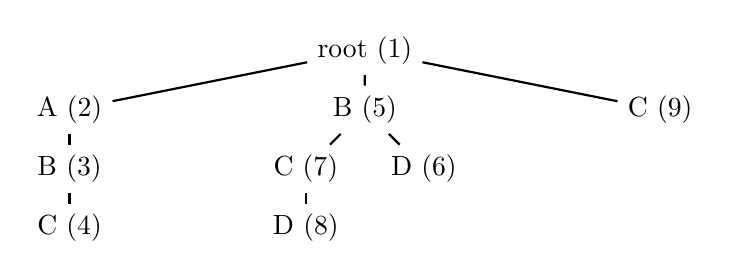
\begin{tikzpicture}
	[thick,scale=0.5, every node/.style={scale=1}]
	\node {root (1)}
	child {node {A (2)}
		child {node {B (3)}
			child {node {C (4)}}
		}
	}	
	child [missing] {}	
	child [missing] {}
	child [missing] {}	
	child [missing] {}	
	child { node {B (5)}
		child {node {C (7)}
			child {node {D (8)}}
		}
		child [missing] {}
		child {node {D (6)}
		}
	}	
	child [missing] {}	
	child [missing] {}
	child [missing] {}	
	child [missing] {}	
	child { node {C (9)} };
	\end{tikzpicture}

而我们的目标串为\textcolor[rgb]{0,0,1}{$ABCDBC$}。 \par

用$3.3.1$节提到的类似于$Search$的方法在模式串所构建的Trie 树上进行匹配,刚开始会经过\textcolor[rgb]{0,0,1}{$(2)$},\textcolor[rgb]{0,0,1}{$(3)$},\textcolor[rgb]{0,0,1}{$(4)$} 号结点,到了$(4)$号结点后,成功匹配了模式串\textcolor[rgb]{1,0,0}{$ABC$},如果按照原有BF算法的朴素思路,需要退回到根结点重新进行下一次匹配,但是显然这样做的效率太低。这是我们就可以借用KMP中 $next$ 数组的思想,不再是从根结点,而是从Trie 树上的某个点继续开始匹配。 \par

注意到 \textcolor[rgb]{0,0,1}{$(3) \to (4)$} 结点和从根结点到\textcolor[rgb]{0,0,1}{$(5) \to (7)$} 结点同样都是 \textcolor[rgb]{1,0,0}{$BC$},事实上我们可以直接跳到 \textcolor[rgb]{0,0,1}{$(7)$} 号结点进行匹配,然后对 \textcolor[rgb]{0,0,1}{$(8)$} 号叶结点进行匹配,所匹配的\textcolor[rgb]{1,0,0}{$BCD$}也是存在于目标串中的模式串。那么问题在于,这个跳转的过程究竟是怎么确定的,我们可以借鉴KMP算法中的 $next$ 数组:\textbf{我们称 $i$ 匹配失败后继续从 $j$ 开始匹配的情况,则 $j$ 是 $i$ 的 $fail$ (失配)指针。} \par

下面给出 $fail$ 指针的实质含义:\textbf{如果一个点 $i$ 的 $fail$ 指针指向 $j$。那么 $root$ 到 $j$ 的字符串是 $root$ 到 $i$ 的字符串的一个后缀}。举例来讲,$root$ 到 \textcolor[rgb]{0,0,1}{$(7)$} 号结点所组成的字符串\textcolor[rgb]{1,0,0}{$BC$}是 $root$ 到 \textcolor[rgb]{0,0,1}{$(4)$} 号结点所组成的字符串\textcolor[rgb]{1,0,0}{$ABC$}的后缀,但是同时我们也能注意到 $root$ 到 \textcolor[rgb]{0,0,1}{$(9)$} 号结点所组成的字符串\textcolor[rgb]{1,0,0}{$C$}同样也是\textcolor[rgb]{1,0,0}{$ABC$}的后缀,那么显然如果有多个后缀,我们取结点深度最深,也就是最长的那个后缀。知道了 $fail$ 指针的含义,随之而来的就是新的问题:我们应该如何求得每个结点的 $fail$ 指针。\par

一个非常显然的结论是,由于 $fail$ 指针指向的是后缀,所以每一个结点 $i$ 所指向的结点 $j$ 的深度一定严格小于 $i$ (其中 $j$ 有可能指向的是空串,也就是 $root$ 结点。


\begin{itemize}
  \item [1)] 显然,深度为 $1$ 的结点,其 $fail$ 指针指向 $root$ 结点。
  \item [2)] 对于某个结点 $fa$ 通过字符 $k$ 转移到的结点 $i$存在,如果$fa$ 的 $fail$ 指针指向的节点 $j_{fa}$ 同样存在由字符 $k$ 转移到的节点 $j$,那么$fail[i]=j$。由于 $fa$ 节点存在的最长后缀是 $fa_j$ 节点,那么 $i$ 节点存在的后缀的最长的长度也只能是$fa_j$的深度加$1$,也就是以$k$字符为转移时的子节点$j$,这一步总体来说是显然的。 \par
	举例来说,当 $fa$ 结点为 \textcolor[rgb]{0,0,1}{$(3)$} 号结点,其字符串为 \textcolor[rgb]{1,0,0}{$AB$},其最长后缀为 \textcolor[rgb]{1,0,0}{$B$},那么 $fa$ 的 $fail$ 指针指向的结点 $j_{fa}$ 就是 \textcolor[rgb]{0,0,1}{$(5)$} 号结点,\textcolor[rgb]{0,0,1}{$(3)$} 号结点以字符 \textcolor[rgb]{1,0,0}{$C$} 所转移到的结点 $i$ 为 \textcolor[rgb]{0,0,1}{$(4)$} 号结点,而 \textcolor[rgb]{0,0,1}{$(5)$} 号结点 $j_{fa}$ 同样存在由字符 \textcolor[rgb]{1,0,0}{$C$} 转移到的结点 $j$,也就是 \textcolor[rgb]{0,0,1}{$(7)$} 号结点,那么 $fail[4] = 7$
  \item [3)] 此时存在一个显然的例外,如果上一种情况定义的 $j$ 节点并不存在,那么上一种情况的转移就不能无条件继续进行下去。例如 \textcolor[rgb]{0,0,1}{$(7)$} 号结点所构成的字符串 \textcolor[rgb]{1,0,0}{$BC$} 其最长后缀为 \textcolor[rgb]{1,0,0}{$C$},也就是 \textcolor[rgb]{0,0,1}{$(9)$} 号结点,但是 \textcolor[rgb]{0,0,1}{$(7)$} 可以通过字符 \textcolor[rgb]{1,0,0}{$D$} 转移到子结点 \textcolor[rgb]{0,0,1}{$(8)$},而 \textcolor[rgb]{0,0,1}{$(9)$} 号结点并不存在相应的子结点。 \par
为了让上一种情况的转移总是能进行下去,我们定义一种新的转移:当$fa$节点存在并且通过字符 $k$ 转移到的结点 $i$ 不存在时,如果$fa$ 的 $fail$ 指针指向的节点 $j_{fa}$,并且 $j_{fa}$ 由字符 $k$ 转移到的节点为 $j$ ,我们让 $i \gets j$。\par 
	这一步转移看上去和上一步转移非常相似,但是其本质含义是不相同的:\textbf{它的含义是如果第 $2$ 种情况无法让从父亲结点继承下来的最长后缀(也就是最理想情况下的最优后缀)延续下去,我们就转而寻求一个次优的后缀(也就是后缀的后缀)},如果 $j$ 结点原本也不存在,那么这个过程就可以一直递归进行下去,直到找到了真正存在的最优后缀。从而转移 $2$ 不再需要结点 $j$ 存在的条件。
	举例来说:假设 $fa$ 结点为 \textcolor[rgb]{0,0,1}{BCD},其子结点 \textcolor[rgb]{0,0,1}{BCDE} 不存在,但是 $fa_j$ 结点为 \textcolor[rgb]{0,0,1}{CD},其对应的子结点 $j$ $\textcolor[rgb]{0,0,1}{CDE}$存在,那么 $i \gets j$,也即 \textcolor[rgb]{0,0,1}{BCD} 通过字符 $\textcolor[rgb]{0,0,1}{E}$ 转移到的是 \textcolor[rgb]{0,0,1}{CDE},也即 $ \textcolor[rgb]{0,0,1}{BCDE}  \gets  \textcolor[rgb]{0,0,1}{CDE}$。 \par
	这时假设再有一个结点 $u$ 为 \textcolor[rgb]{0,0,1}{ABCD}, $fail[u]=fa$,也即 $fail[\textcolor[rgb]{0,0,1}{ABCD}]=\textcolor[rgb]{0,0,1}{BCD}$。$u$ 存在一个子结点 $v$ 为 \textcolor[rgb]{0,0,1}{ABCDE},本来由于这种转移 $2$ 因为 \textcolor[rgb]{0,0,1}{BCDE} 不存在而无法进行下去,但由于新加入了转移 $3$,此时 $fail[\textcolor[rgb]{0,0,1}{ABCDE}] = (\textcolor[rgb]{0,0,1}{BCDE} \gets \textcolor[rgb]{0,0,1}{CDE}) = \textcolor[rgb]{0,0,1}{CDE}$。这也印证了上面的说法:如果我们不能找到一个最优的后缀\textcolor[rgb]{0,0,1}{BCDE},我们转而寻找 \textcolor[rgb]{0,0,1}{BCDE} 存在的后缀,也即次优的后缀。

\end{itemize}

概括上述过程,可以总结为,如果一个结点存在,那么使用转移 $2$,如果一个结点不存在(但是它的父亲存在),那么使用转移 $3$。由于求一个结点的 $fail$ 时,其父亲结点的 $fail$ 必须要已经求出,由最开头那个显然的结论,我们使用 BFS 遍历树,按照深度递增依次求出每个结点的 $fail$。 \par

获得 $fail$ 指针的具体伪代码见下文\textbf{算法6}:

\begin{algorithm}
\caption{Get-Fail}  
\label{alg: Aho-Corasick Automaton Get-Fail} 
\begin{algorithmic} [1] 
	\Require $root$: Trie-Tree root
	\Ensure $fail[]$: Fail Array
    \Function {Get-Fail}{$root$, $fail[]$}
		\For{$i = 0 \to K - 1$}
			\State $Null.children[i] = root$ Make sure node which not exists still could back to root 
		\EndFor
		\State \textbf{Queue} $Q$
		\State $fall[root] \gets Null$
		\State \Call{Push} {Q, root}
		\While { \textbf{not} \Call{Is-Empty}{Q}}
			\State \Call{Pop}{Q, fa}
			\For{$k = 0 \to K - 1$} : K is the size of Character-set
				\State $i \gets fa.children[k]$
				\State $fa_j \gets fail[fa]$
				\State $j \gets fa_j.children[k]$
				\If {$i \ne Null$} Case (2)
					\State $fail[i] \gets j$
					\State \Call{Push} {Q, i}
				\Else: Case (3)
					\State $fa.children[k] \gets j$
				\EndIf
			\EndFor
		\EndWhile
	\EndFunction  
\end{algorithmic}
\end{algorithm}

求出 $fail$ 指针之后,查询就简单了。为避免重复计算,我们对每个经过的结点打上 $vis$ 标记。

同时,如果一个字符串匹配成功,那么他的 $fail$ (后缀) 也必定匹配成功。于是我们以 $fail$ 指针为链一直向根节点跳转,打上 $vis$ 标记的同时统计答案。

查询的具体伪代码见下文\textbf{算法7}:

\begin{algorithm}
\caption{Query}  
\label{alg: Aho-Corasick Automaton Query} 
\begin{algorithmic} [1] 
	\Require $root$: Trie-Tree Root; $fail[]$: Fail Array; $S$: Target String
	\Ensure $Ans$: Total Matched Pattern Strings
    \Function {Query}{$root$, $fail[]$, $S$}
		\State $Ans \gets 0$
		\State $u \gets root$
		\For{$i = 0 \to $ \Call{Length}{S} $-1$}
			\State $v \gets u.children[$ \Call{CharToIndex}{S[i]} $]$
			\While {$v \ne root$ \textbf{and} \textbf{not} $vis[v]$}
				\State $Ans += 1$
				\State $vis[v] \gets True$
				\State $v = fail[v]$
			\EndWhile
			\State $v \gets u.children[$ \Call{CharToIndex}{S[i]} $]$
		\EndFor
		\State \Return $Ans$
	\EndFunction  
\end{algorithmic}
\end{algorithm}

\subsubsection {算法分析}

首先来分析Aho-Corasick Automaton 算法的时间复杂度:假设有 $N$ 个模式串,平均长度为 $L$;目标串长度为 $M$。 建立Trie树:$\mathcal{O}(N \cdot L)$ 建立$fail$ 指针:$\mathcal{O}(N \cdot L)$ 模式匹配:$\mathcal{O}(M \cdot L)$。\par
所以,总时间复杂度为: $\mathcal{O}((N+M) \cdot L)$

至此,单目标串多模式串的匹配问题已经相对解决,上述的时间复杂度也相对优越,但Aho-Corasick Automaton 算法仍有其局限性:\textbf{和KMP算法一样,算法需要初始化的是模式串$T$而不是目标串$S$}。这意味着对于多模式串来说,它是离线算法而不是在线算法,每当新加入一个模式串的时候,我们仍需要重新初始化一遍所有的 $fail$ 指针,并重新进行一遍模式匹配。在后面几章的后缀系算法中,这个问题就能得到很好的解决。Aho-Corasick Automaton 算法最重要的,也还是其有关 $fail$ 指针的思想,$fail$ 指针本身构成了一棵树,$fail$ 指针和父亲指针又构成了 DAG,就可以在上面和DP等思想结合,限于篇幅在这里就不再展开详述。

另一个值得注意的有意思的事情是,目标串的Trie 树退化成单链的情况,和KMP算法有着千丝万缕的联系。

\subsection {后缀树}

\subsubsection {算法描述}

假设存在一个目标串\textcolor[rgb]{0,0,1}{$BANANAS$}。回到$3.3.2$节中提出的思路,我们将其的每个后缀插入到Trie 树中。得到的结果如下图所示: \par

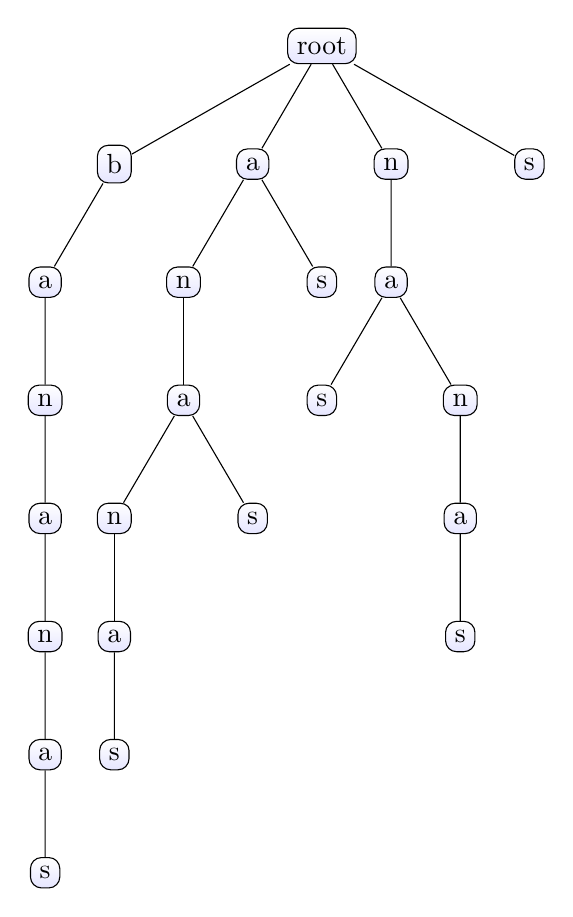
\begin{tikzpicture}[sibling distance=5em,
  every node/.style = {shape=rectangle, rounded corners,
    draw, align=center,
    top color=white, bottom color=blue!10}]]
  \node {root}
    child { node {b} 
		child { node {a} 
			child { node {n} 
				child { node {a} 
				child { node {n}
						child { node {a} 
						child { node {s} }
					}
					}
				}
			}
		}
		child[missing] {}
	}
    child { node {a}
		child { node {n}
		child { node {a}
			child { node {n}
						child { node {a} 
						child { node {s} }
					}
			}
			child { node {s} } 
		}
		}
		child { node {s} }}
		child { node {n} child {node {a} 
			child { node {s} } 
			child { node {n}
						child { node {a} 
						child { node {s} }
					}
			}
		}
		}
		child { node {s} };
\end{tikzpicture}

可以看到的是,得到的 Trie 树结点数量达到了 $\mathcal{O}(N ^ 2)$ 的程度。然而,像 \textcolor[rgb]{0,0,1}{BANANAS} 这样只有单链的分支,完全可以\textbf{将整个树链压缩成一个字符串存在一个结点里}。准确的来说:如果结点 $v$ 到其祖先 $u$ 的路径中的结点(包括 $u$ 但不包括 $v$)除了路径本身没有与其他任何边相连,我们就将路径 $u \to v$ 所构成的子串存在一个新的结点中,并将这个结点的父亲设为原来 $u$ 的父亲,孩子设为原来 $v$ 的孩子。压缩后的Trie 树也即后缀树,如下图所示: \par

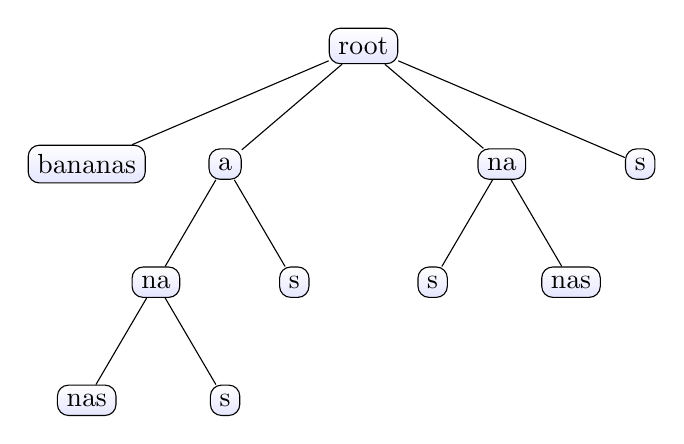
\begin{tikzpicture}[sibling distance=5em,
  every node/.style = {shape=rectangle, rounded corners,
    draw, align=center,
    top color=white, bottom color=blue!10}]]
  \node {root}
    child { node {bananas} }
    child { node {a} 
		child { node {na}
			child { node {nas} }
			child { node {s} } 
		}
		child { node {s} }}
		child[missing] {}
		child { node {na} 
			child { node {s} } 
			child { node {nas} } 
		} 
		child { node {s} };
\end{tikzpicture}

可以证明,此时结点的数量在 $\mathcal{O}(N)$ 的级别。

记 $str(x)$ 为结点 $x$ 上的从根结点到当前结点连成的字符串,可以发现路径压缩之后,每个结点 $x$ 表示了原目标串 $S$ 中的多个连续子串。记其中最短的长度为 $lowest(x)$,最长的长度为 $largest(x)$,那么 $x$ 所管辖的字符串为 $str(x)$ 长度在 $[lowest(x), largest(x)]$ 的前缀。不难发现 $largest(x)=length(str(x))$,$lowest(x)=largest(fa_x)$。那么记 $S_x$ 为这些子串的集合,则 $S$ 的任意子串属于且仅属于一个集合。

由此已经可以分析出后缀树的许多性质。记 $startpos(x)$ 为子串 $t$ 在 $S$ 中所有出现位置开始位置的集合,例如 $startpos(\textcolor[rgb]{0,0,1}{CB})=\{ 1, 3 \}$,那么 $startpos(t_1) = startpos(t_2)$ ,当且仅当 $t_1$ 和 $t_2$ 属于同一个 $S_x$。不妨设 $ss(x)$ 为结点 $x$ 表示的任意字符串,那么 $startpos(ss(x)) \in startpos(ss(fa_x))$,若 $x$,$y$ 不存在祖先关系,则 $startpos(x) \cap startpos(y) = \phi$。

\subsubsection {算法分析}

尽管我们现在还不知道怎么建出后缀树,但是假设我们已经有了一棵建好的后缀树,我们就已经能解决许多问题。最直观的是,由于后缀树建立的是目标串 $S$ 的信息,所以此时我们已经能在 $\mathcal{O}(N)$ 的空间复杂度下,以$\mathcal{O}(M)$ 的时间复杂度在线地解决模式串匹配的问题。而后缀树上述提到的性质也能作为有力的工具解决很多问题,例如\textbf{给定一个长度为 $N$ 的字符串 $S$,共有 $M$ 个询问,每个询问求解 $S$ 从 $a$ 到 $b$ 的子串和从 $c$ 到 $d$ 的子串的最长公共前缀的长度的最大值。} \par

令 $T_i$ 表示 $S$ 从第 $i$ 个字符开始的后缀,那么问题等价于求 $min(d-c+1,max_{a \leq k \leq b}(lcp(T_k, T_d))$。二分答案 $ans$,在后缀树上从后缀 $d$ 所在的结点往上跳到 $ans \leq largest(x)$ 且深度最深的结点 $x$,那么我们只需要查询结点 $x$ 的子树中是否存在 $[c+ans-1,d]$ 范围内的后缀。我们每个结点开一棵权值线段树,启发式合并就解决了问题。 \par

可以发现建出后缀树和得到相关信息以后,用DP或者数据结构维护后缀乃至子串的信息会变得非常方便。 \par

后缀树本身作为一种数据结构,在ACM竞赛中一般不常使用,ACM竞赛中一般使用后缀数组(Suffix Array)或者后缀自动机(Suffix Automaton)。在后缀数组或者后缀自动机建立完成之后,其中自然包含了一棵建立好的后缀树,接下来的章节介绍的就是后缀自动机算法。

\subsection {Suffix Automaton 算法}

\subsubsection {算法描述}

对给定字符串 $S$ 的后缀自动机是一个最小化确定有限状态自动机,它能够接收字符串 $S$ 的所有后缀。其是一个有向无环连通图, $V$ 集合表示状态(当前所匹配完成的字符串),$E$ 表示转移(下一个匹配的字符)。某一状态 $T_0$ (空集)被称为初始状态,由它能够到达其余所有状态。 \par

一个或多个状态被标记为终止状态。如果我们从初始状态 $T_0$ 经由任意路径走到某一终止状态,并顺序写出所有经过边的标记,得
到的字符串必然是 $S$ 的某一后缀。 \par

在符合上述诸条件的所有自动机中,后缀自动机有最少的顶点数。 \par

考虑字符串 $S$ 的任意非空子串t。我们称终点集合 $endpos(t)$ 为:\textbf{$S$ 中所有是 $T$ 出现位置终点的集合。} \par

我们称两个子串 $t_1$ 和 $t_2$“终点等价”,如果它们的终点集合一致:$endpos(t_1)=endpos(t_2)$。因此,所有 $S$ 的非空子串可以根据终点等价性分成若干类。 \par

事实上对后缀自动机,终点等价字符串仍然保持相同性质。换句话说,后缀自动机中状态数等价于所有子串的终点等价类个数,加上初始状态。每个状态对应一个或多个拥有相同终点集合的子串。 \par

关于终点集合,我们给出一些简单但重要的事实。 \par

\begin{itemize}
  \item [1)] 
\textbf{引理1}:两个非空子串 $u$ 和 $v$ ($length(u) \leq length(v)$)是终点等价的,当且仅当 $u$ 在字符串 $S$ 中仅作为 $w$ 的后缀出现。
  \item [2)] 
\textbf{引理2}:考虑两个非空子集 $u$ 和 $v$ ($length(u) \leq length(v)$)。它们的终点集合不相交,或者 $endpos(w)$ 是 $endpos(u)$ 的子集。进一步地,这取决于 $u$ 是否是 $w$ 的后缀。
 \item [3)] 
\textbf{引理3}:考虑一个终点等价类。将该等价类中的子串按长度递减排序。排序后的序列中,每个子串将比上一个子串短,从而是上一个字串的后缀。换句话说,某一终点等价类中的字符串互为后缀,它们的长度依次取区间 $[x,y]$ 内的所有数。
\end{itemize}

考虑一个状态 $v \ne t_0$。就我们目前所知,有一个确定的子串集合,其中元素和 $v$ 有着相同的终点集合。并且,如果我们记 $w$ 是其中的最长者,其余子串均是 $w$ 的后缀。我们还知道 $w$ 的前几个后缀(按照长度降序)在同一个终点等价类中,其余后缀(至少包括空后缀)在别的终点等价类中。令 $t$ 是第一个这样的后缀,对它我们建立后缀链接。换言之,$v$ 的后缀链接 $link(v)$ 指向在不同等价类中的 $w$ 的最长后缀。

\subsubsection {算法分析}

可以发现后缀树的 $startpos(x)$ 和后缀自动机的 $endpos(x)$ 存在$startpos(x)=rev(endpos(x))$的关系。也就是说原串的后缀树是反串后缀自动机建出的后缀链接。我们就可以用后缀自动机在 $\mathcal{O}(N)$ 的复杂度内建出后缀树,并处理后缀树相关的问题。\par

此外更棒的是,利用后缀自动机建立后缀树的过程是在线的,我们可以随时往目标串 $S$ 末尾添加新的字符构建新的后缀自动机和后缀树,并且时间复杂度也是线性的。那么,我们现在解决模式串匹配的问题,既可以对模式串 $T$ 做到在线线性,又可以对目标串 $S$ 做到在线线性。\textbf{至此我们可以说,模式串匹配的问题已经被我们完美解决。}

\section{总结}

在这篇论文中,我们对模式串匹配问题的各种算法进行了研究。最开始的 \textbf{Brute-Force算法} 只能在 $\mathcal{O}(N \cdot M)$ 的复杂度下解决问题,\textbf{Knuth-Morris-Pratt算法}则可以优化到单次单模式匹配的复杂度是 $\mathcal{O}(N + M)$ 。\textbf{Aho-Corasick Automaton算法}可以对多模式串匹配问题是线性复杂度,但是对模式串 $T$ 和 目标串 $S$ 都是离线的。\textbf{Suffix Tree算法}构建成功后,可以做到对模式串 $T$ 在线,但如果以\textbf{Suffix Automaton算法}的形式构建后缀树的话,则既可以对模式串 $T$ 做到在线线性,又可以对目标串 $S$ 做到在线线性。综上所述,我们对不同层次的算法都进行了总结,并在最后完美的解决了问题。 \par

虽然复杂度各有优劣,但是不同算法的思想都值得我们学习。无论是\textbf{Knuth-Morris-Pratt算法} 中的 $next$ 指针还是\textbf{Aho-Corasick Automaton算法}中的 $fail$ 指针,抑或是\textbf{Suffix Automaton算法}中的后缀链接,有时利用这些思想,才是解出ACM题目的关键。

\section{参考文献}

\begin{itemize}
 \item [[1]] 
http://www.ruanyifeng.com/blog/2013/05/Knuth%E2%80%93Morris%E2%80%93Pratt_algorithm.html
\item [[2]] 
https://blog.csdn.net/dark\_cy/article/details/88698736
\item [[3]] 
https://blog.csdn.net/shiqining888/article/details/25818029
\item [[4]] 
https://blog.csdn.net/qq\_21201267/article/details/93513683
\item [[5]] 
https://www.cnblogs.com/hyfhaha/p/10802604.html
\end{itemize}

\end{document}